\documentclass[xcolor={dvipsnames}]{beamer}
\usepackage[utf8]{inputenc}

\usepackage{amsmath}
\usepackage{graphicx}  % For including graphics
\usepackage{subcaption} % For subfigures
\usepackage{caption}   % For customizing captions

\captionsetup[figure]{
  name=,
  singlelinecheck=off,
  labelsep=colon,
  labelfont=bf,
  font=footnotesize,
  justification=centering,
}

\captionsetup[table]{
  name=,
  singlelinecheck=off,
  labelsep=colon,
  labelfont=bf,
  font=normal,
  justification=centering,
}

\usetheme{Madrid}
\usecolortheme{default}
\setbeamertemplate{enumerate items}[default]
\setbeamercolor*{structure}{bg=white,fg=black}

% \setbeamercolor*{palette primary}{use=structure,fg=white,bg=structure.fg}
% \setbeamercolor*{palette secondary}{use=structure,fg=white,bg=structure.fg!75}
% \setbeamercolor*{palette tertiary}{use=structure,fg=white,bg=structure.fg!50!black}
% \setbeamercolor*{palette quaternary}{fg=white,bg=black}

% \setbeamercolor{section in toc}{fg=black,bg=white}
% \setbeamercolor{alerted text}{use=structure,fg=structure.fg!50!black!80!black}
% \setbeamercolor{frametitle}{bg=black,fg=white}

% \setbeamercolor{titlelike}{parent=palette primary,fg=structure.fg!50!black}
% \setbeamercolor{frametitle}{bg=gray!10!white,fg=black}

% \setbeamercolor*{titlelike}{parent=palette primary}

% \setbeamercolor{block title example}{bg=black,fg=white}

% \usepackage{times,url}

% \setbeamertemplate{footline}[frame number]
% \setbeamertemplate{footline}[frame number]{}

\setbeamertemplate{footline}{}

\setbeamertemplate{footline}
% {
%   \leavevmode%
%   \hbox{%
%   \begin{beamercolorbox}[wd=.333333\paperwidth,ht=2.25ex,dp=1ex,center]{author in head/foot}%
%     \usebeamerfont{author in head/foot}\insertsection
%   \end{beamercolorbox}%
%   \begin{beamercolorbox}[wd=.333333\paperwidth,ht=2.25ex,dp=1ex,center]{title in head/foot}%
%     \usebeamerfont{title in head/foot}\insertsubsection
%   \end{beamercolorbox}%
%   \begin{beamercolorbox}[wd=.333333\paperwidth,ht=2.25ex,dp=1ex,right]{date in head/foot}%
%     \usebeamerfont{date in head/foot}\insertshortdate{}\hspace*{2em}
%     \insertframenumber{} / \inserttotalframenumber\hspace*{2ex} 
%   \end{beamercolorbox}}%
%   \vskip0pt%
% }

%------------------------------------------------------------
%This block of code defines the information to appear in the
%Title page
\title[About Beamer] %optional
{Interstellar Interceptors}

\subtitle{Mission design for rendezvous with objects in hyperbolic orbits}

\author[Martínez, Jorge] % (optional)
{
    Jorge Martínez\\
    \vspace{1cm}
    Supervised by:\\
    \vspace{0.5cm}
    Josep M. Trigo-Rodríguez (ICE-CSIC/IEEC)\\
    Eloy Peña-Asensio (Politecnico di Milano)\\
    \vspace{0.5cm}
    \footnotesize{Universidad Internacional de Valencia}
}

\vspace{-0.5cm}
\date{May 22, 2024}

% \logo{\includegraphics[height=1cm]{overleaf-logo}} 

%End of title page configuration block
%------------------------------------------------------------



%------------------------------------------------------------
%The next block of commands puts the table of contents at the 
%beginning of each section and highlights the current section:

\AtBeginSection[]
{
  \begin{frame}
    \frametitle{Table of Contents}
    \tableofcontents[currentsection]
  \end{frame}
}
%------------------------------------------------------------


\begin{document}

%The next statement creates the title page.
\frame{\titlepage}

%---------------------------------------------------------
\begin{frame}
\frametitle{What are interstellar objects?}

\begin{block}{Definition}
    Interstellar objects (ISOs) are asteroids, comets or planetary bodies moving
    through interstellar medium (ISM) without being gravitationally bound to a
    star.
\end{block}

\begin{figure}[h]
    \centering
    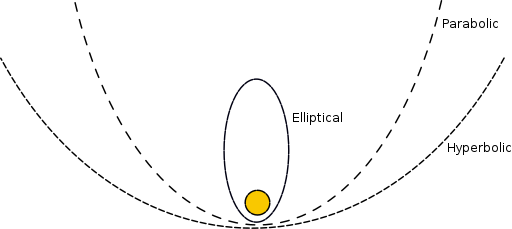
\includegraphics[width=0.75\textwidth]{fig/static/orbits.png}
    \caption{ISOs follow hyperbolic orbits}
    \label{fig:example_figure}
\end{figure}

\end{frame}
%---------------------------------------------------------

%---------------------------------------------------------
\begin{frame}
\frametitle{Why are interstellar objects important?}

They present a unique opportunity to study extraterrestrial bodies that have
traversed vast cosmic distances.\\[0.5cm]

\pause

Their study can unleash information about:\\[0.5cm]

\begin{itemize}
    \item Better understanding the formation of planetary systems
    \item Exploring their physical and chemical composition
    \item Technological motivation
\end{itemize}

\pause

    \vspace{0.5cm}
    \begin{alertblock}{Motivation of this work}
    \vspace{0.2cm}
    Design orbits for rendezvous with ISOs to study their physical properties.
    \vspace{0.2cm}
\end{alertblock}

\end{frame}
%---------------------------------------------------------

%---------------------------------------------------------
\begin{frame}
\frametitle{Discovered interstellar objects}

There are two confirmed ISOs to this day:

\begin{figure}
    \centering
    \begin{minipage}{0.45\textwidth}
        \centering
        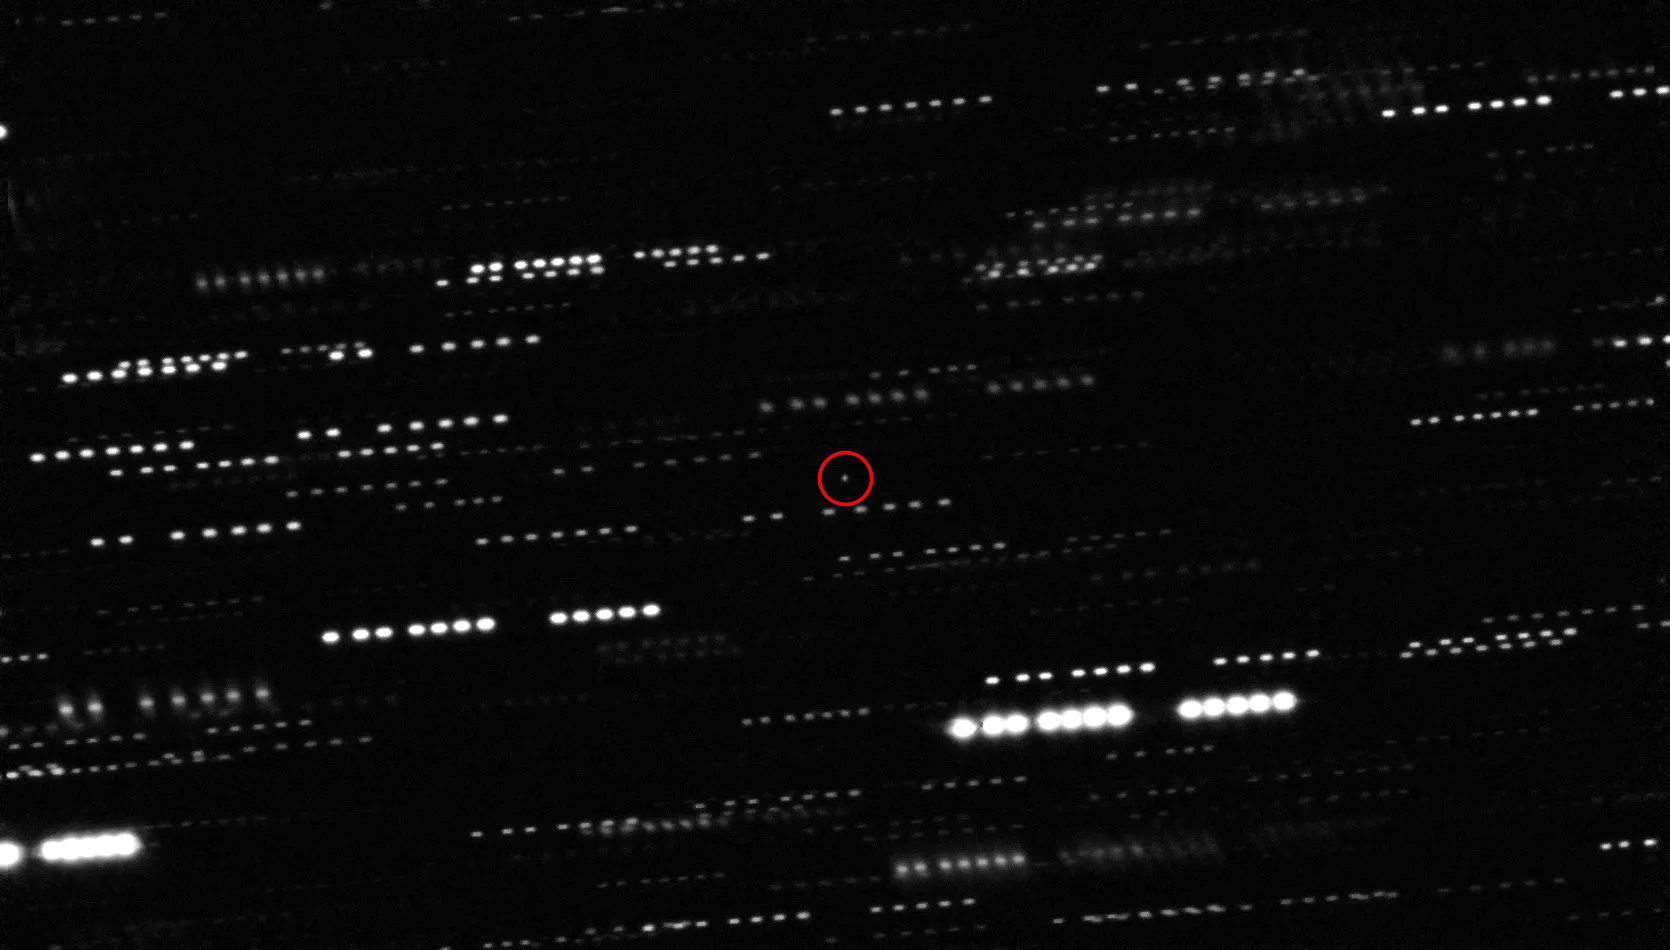
\includegraphics[width=\textwidth]{fig/static/oumuamua/shape.png}
            \caption{1I/'Oumuamua\\[0.25cm]\tiny{ESO's VLT and GST Telescopes}}
        \label{fig:figure1}
    \end{minipage}
    \hfill
    \begin{minipage}{0.45\textwidth}
        \centering
        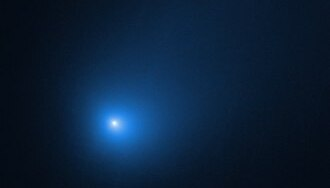
\includegraphics[width=\textwidth]{fig/static/borisov/shape.jpg}
            \caption{2I/Borisov\\[0.25cm]\tiny{NASA Hubble Space Telescope}}
        \label{fig:figure2}
    \end{minipage}
\end{figure}

\pause
\vspace{-0.25cm}
These interlopers present the following orbit attributes:
\vspace{0.1cm}

\begin{itemize}
    \item Hyperbolic orbits
    \item High relative velocity w.r.t. the Sun
    \item Random inclination
    \item Discovered close to the direction of the Solar Apex
\end{itemize}

\end{frame}
%---------------------------------------------------------

%---------------------------------------------------------
\begin{frame}
\frametitle{Orbits of 1I/'Oumuamua and 2I/Borisov}

\begin{figure}
    \centering
    \begin{minipage}{0.45\textwidth}
        \centering
        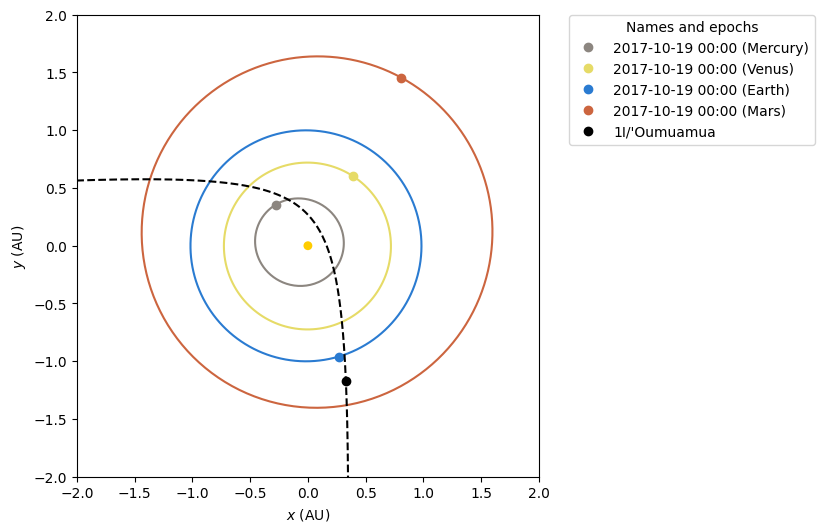
\includegraphics[width=0.9\textwidth]{fig/static/oumuamua/orbit_xy.png}
        \caption{1I/'Oumuamua orbit top view}
        \label{fig:figure1}
    \end{minipage}
    \hfill
    \begin{minipage}{0.45\textwidth}
        \centering
        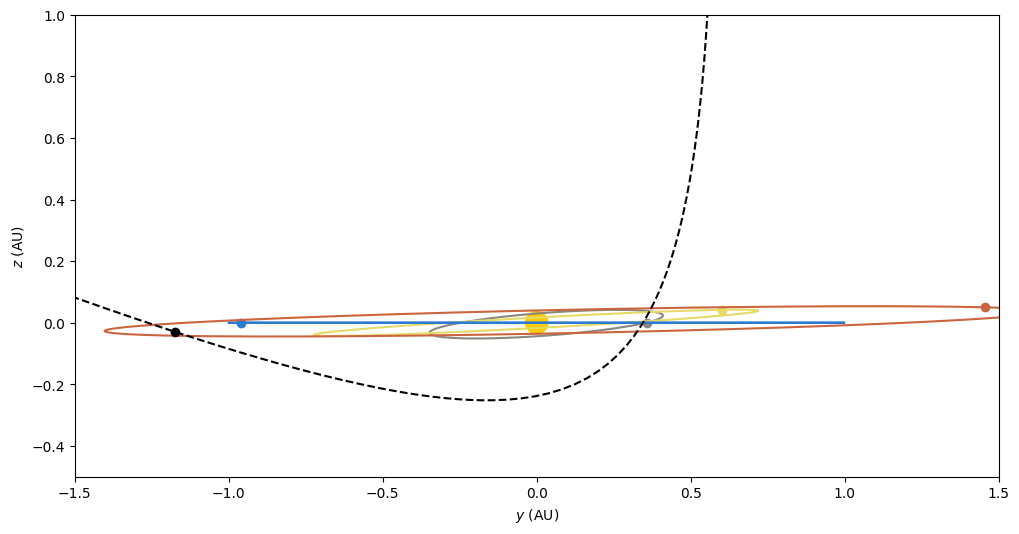
\includegraphics[width=0.9\textwidth]{fig/static/oumuamua/orbit_yz.png}
        \caption{1I/'Oumuamua orbit side view}
        \label{fig:figure2}
    \end{minipage}
\end{figure}

\vspace{-0.35cm}

\begin{figure}
    \centering
    \begin{minipage}{0.45\textwidth}
        \centering
        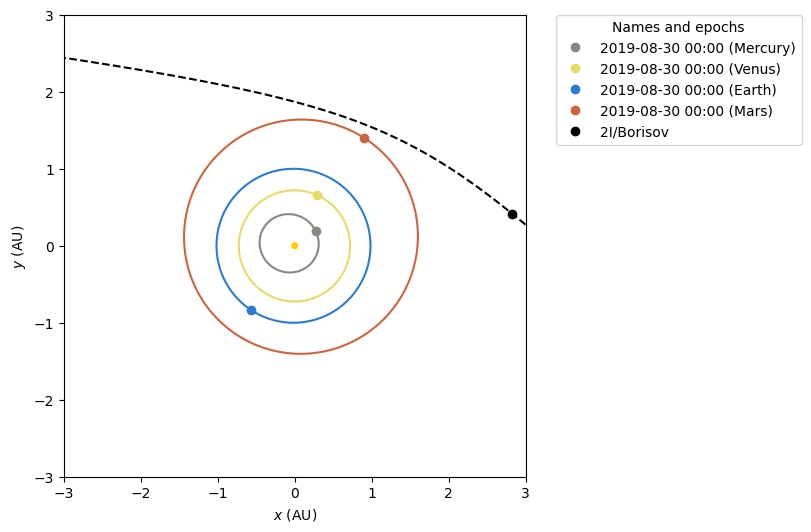
\includegraphics[width=0.9\textwidth]{fig/static/borisov/orbit_xy.png}
        \caption{2I/Borisov orbit top view}
        \label{fig:figure1}
    \end{minipage}
    \hfill
    \begin{minipage}{0.45\textwidth}
        \centering
        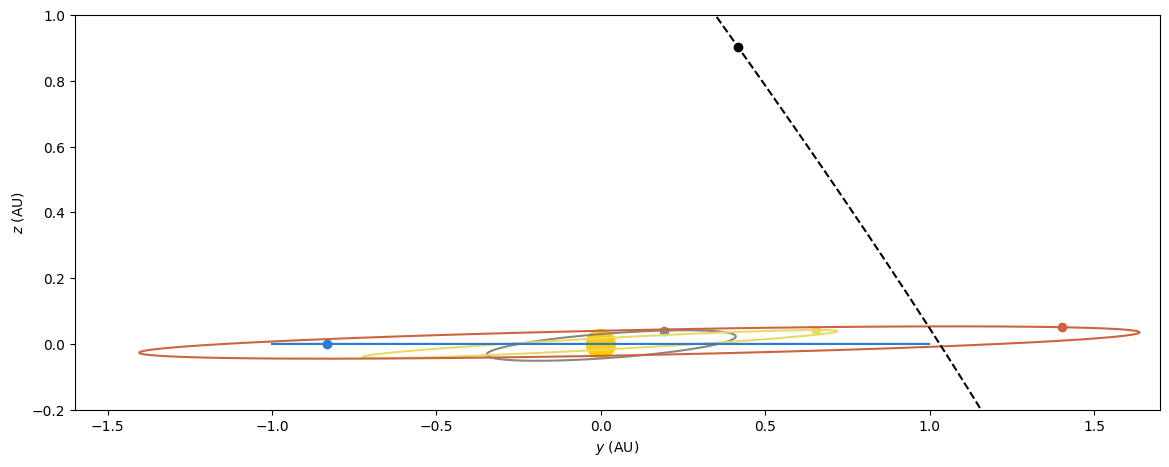
\includegraphics[width=0.9\textwidth]{fig/static/borisov/orbit_yz.png}
        \caption{2I/Borisov orbit side view}
        \label{fig:figure2}
    \end{minipage}
\end{figure}

\end{frame}
%---------------------------------------------------------


%---------------------------------------------------------
\begin{frame}
\frametitle{Navigating through space: the Lambert's problem}

Lambert's problem is the Boundary Value Problem (BVP) in the context of the
restricted two-body problem dynamics.

\begin{columns}

  \column{0.5\textwidth}

    \begin{figure}[h]
        \centering
        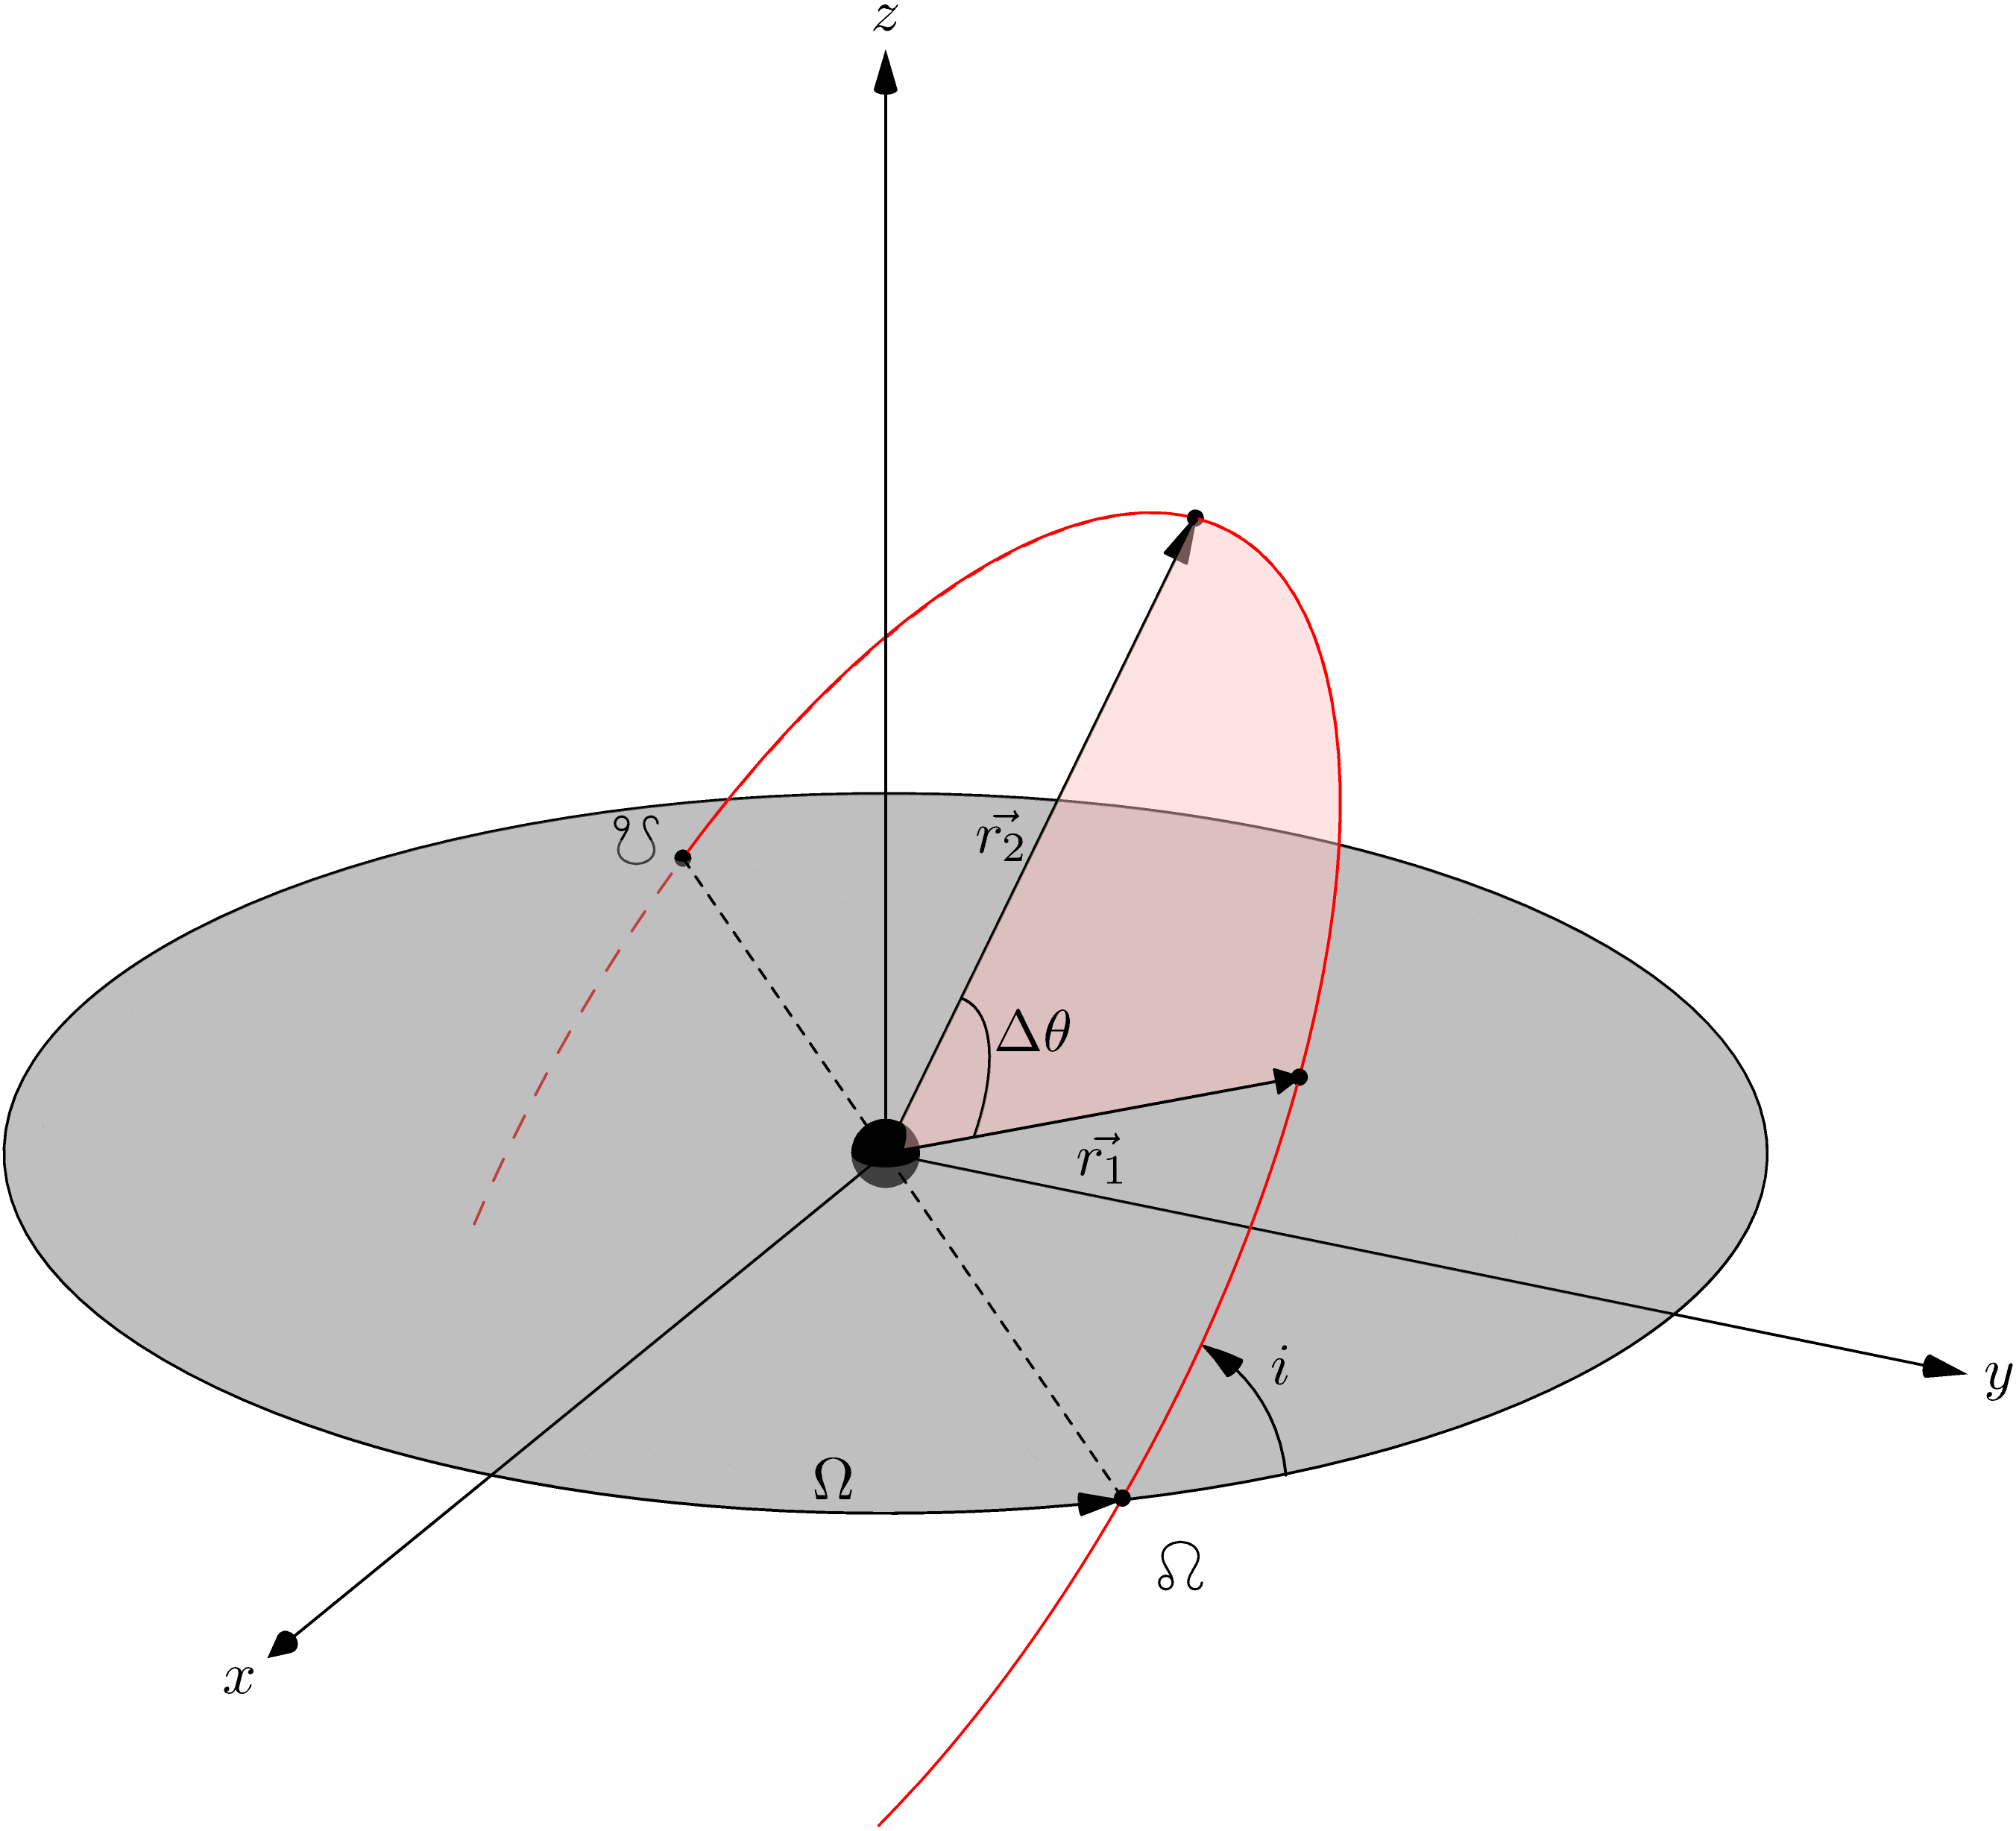
\includegraphics[width=0.85\textwidth]{fig/lambert-problem/geometry.png}
        \caption{Geometry of the Lambert's problem}
        \label{fig:example_figure}
    \end{figure}
  
  \column{0.5\textwidth}

  $$\ddot{\vec{r}} = -\frac{\mu}{r^3}\vec{r} \quad \begin{cases}
     & \vec{r}\;(t_1) = \vec{r_1} \\ 
     & \vec{r}\;(t_2) = \vec{r_2}
     \end{cases}$$


\pause

\vspace{1cm}
Solve for the orbit which passes through $\vec{r_1}$ and $\vec{r_2}$ over a
finite amount of time $\Delta t = t_2 - t_1$.

\end{columns}

\end{frame}
%---------------------------------------------------------

%---------------------------------------------------------
\begin{frame}
\frametitle{Estimating the cost of the maneuver using the $C_3$ energy}

Lambert's problem computes the initial velocity $\vec{v_1}$ and final velocity
$\vec{v_2}$ of the orbit.

\vspace{0.25cm}
    \begin{itemize}
        \item First impulse: $\Delta v_1 = \left \|  v_{1} - v_{\text{origin}} \right \|$
        \item Last impulse: $\Delta v_2 = \left \|  v_{2} - v_{\text{iso}} \right \|$
    \end{itemize}
\vspace{0.25cm}

\pause
The total cost of the maneuver is $\Delta v = \Delta v_1 + \Delta v_2$. This
relates with the fuel mass via the Tsiolkovsky rocket equation:

$$ \Delta v = v_{e} \ln \left( \frac{m_0}{m_f} \right) $$

\pause
\vspace{0.25cm}
The characteristic energy for hyperbolic orbits $C_3$ is defined as:

$$ C_3 = v_{\infty}^2 $$

\end{frame}
%---------------------------------------------------------

%---------------------------------------------------------
\begin{frame}
\frametitle{Modern launching technologies}

\begin{figure}[h]
    \centering
    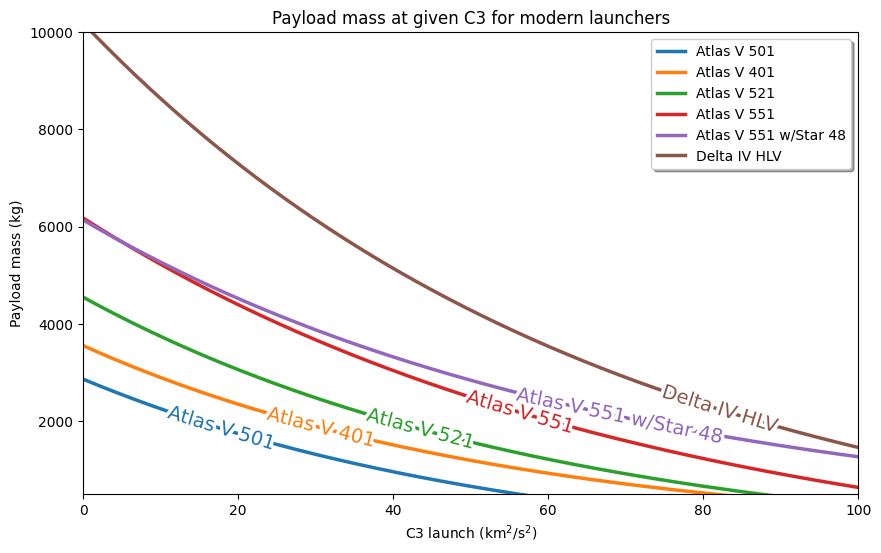
\includegraphics[width=\textwidth]{fig/static/payload_vs_c3.png}
    \caption{Maximum payload mass vs. $C_3$ energy for different launchers}
    \label{fig:payload_vs_c3}
\end{figure}

\end{frame}
%---------------------------------------------------------

%---------------------------------------------------------
\begin{frame}
\frametitle{Minimizing the cost of the maneuver}

Porkchop plots are used to find the optimal launch and arrival dates by solving
Lambert's problem for a variety of trajectories.

\pause

\begin{figure}[h]
    \centering
    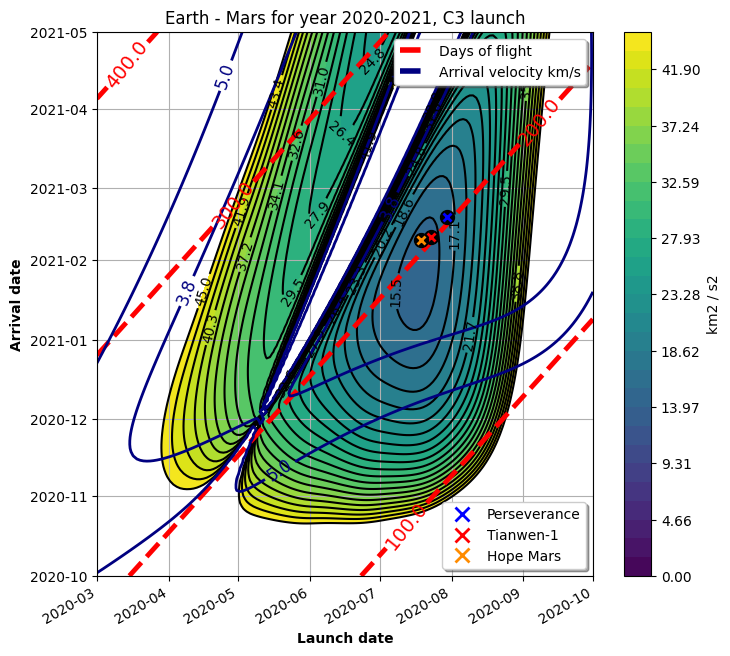
\includegraphics[width=0.6\textwidth]{fig/static/porkchop.png}
    \caption{Porkchop plot between Earth and Mars}
    \label{fig:porkchop}
\end{figure}

\end{frame}
%---------------------------------------------------------

%---------------------------------------------------------
\begin{frame}
\frametitle{Analyzed scenarios}

The analyzed scenarios in this work for each discovered ISO include:

\vspace{0.25cm}
\begin{itemize}
    \item Direct transfer between the Earth and the ISO
    \item Direct transfer between the L2 point and the ISO
\end{itemize}

\pause

\begin{figure}[h]
    \centering
    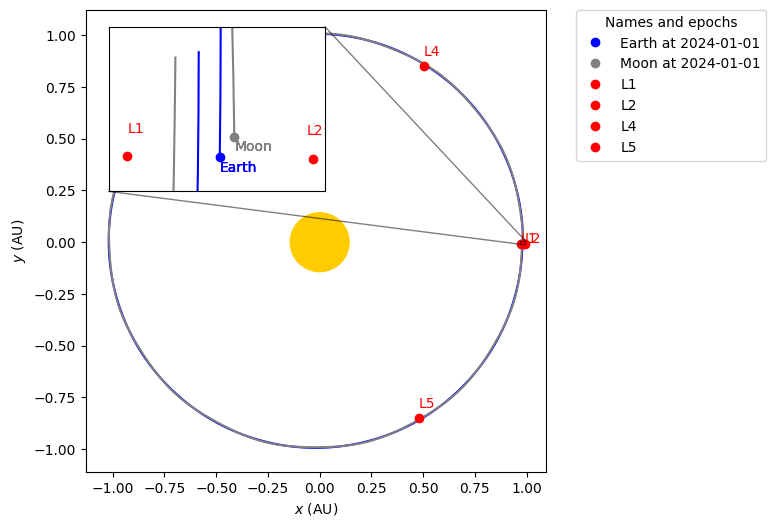
\includegraphics[width=0.6\textwidth]{fig/static/lagrange_points.png}
    \caption{Lagrange points for the Sun Earth-Moon system}
    \label{fig:lagrange}
\end{figure}

\end{frame}
%---------------------------------------------------------

%---------------------------------------------------------
\begin{frame}
\frametitle{1I/'Oumuamua: direct prograde transfer from Earth}

\begin{figure}[h]
    \centering
    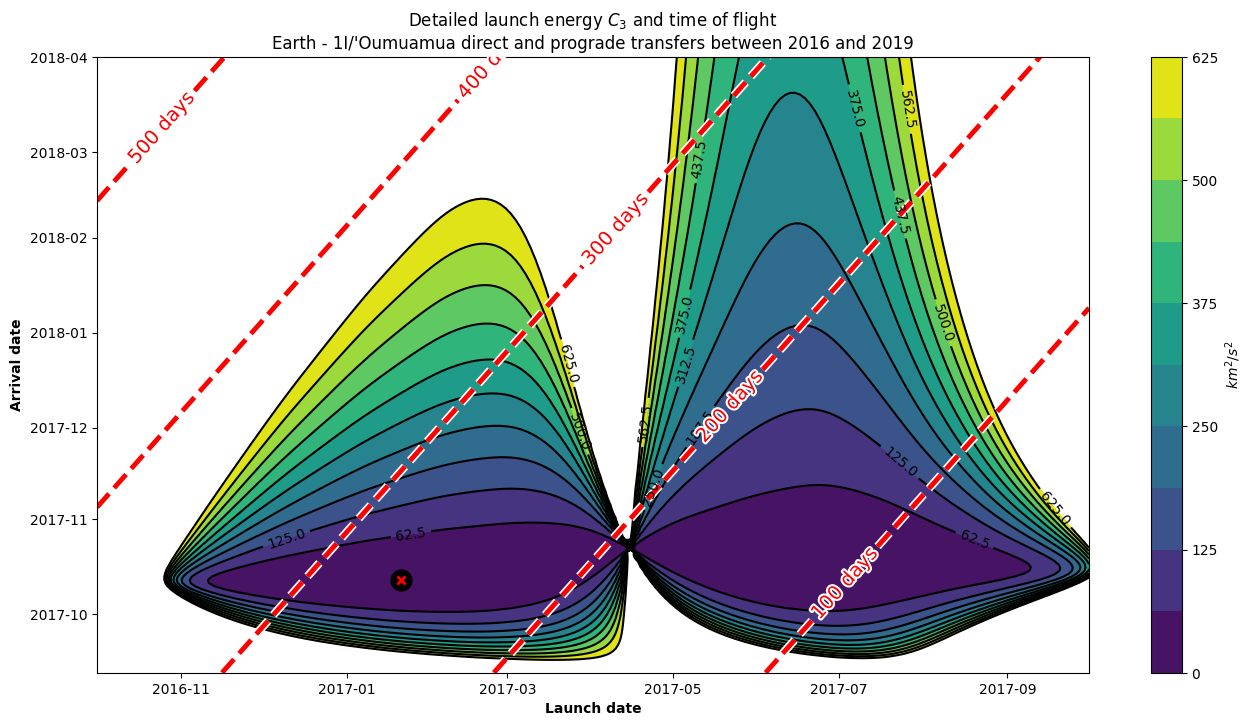
\includegraphics[width=\textwidth]{fig/static/oumuamua/direct-detailed-porkchop-tof.png}
    \caption{Direct transfer from Earth}
    \label{fig:oumuamua-earth-transfer}
\end{figure}

\end{frame}
%---------------------------------------------------------

%---------------------------------------------------------
\begin{frame}
\frametitle{1I/'Oumuamua: direct prograde transfer from L2}

\begin{figure}[h]
    \centering
    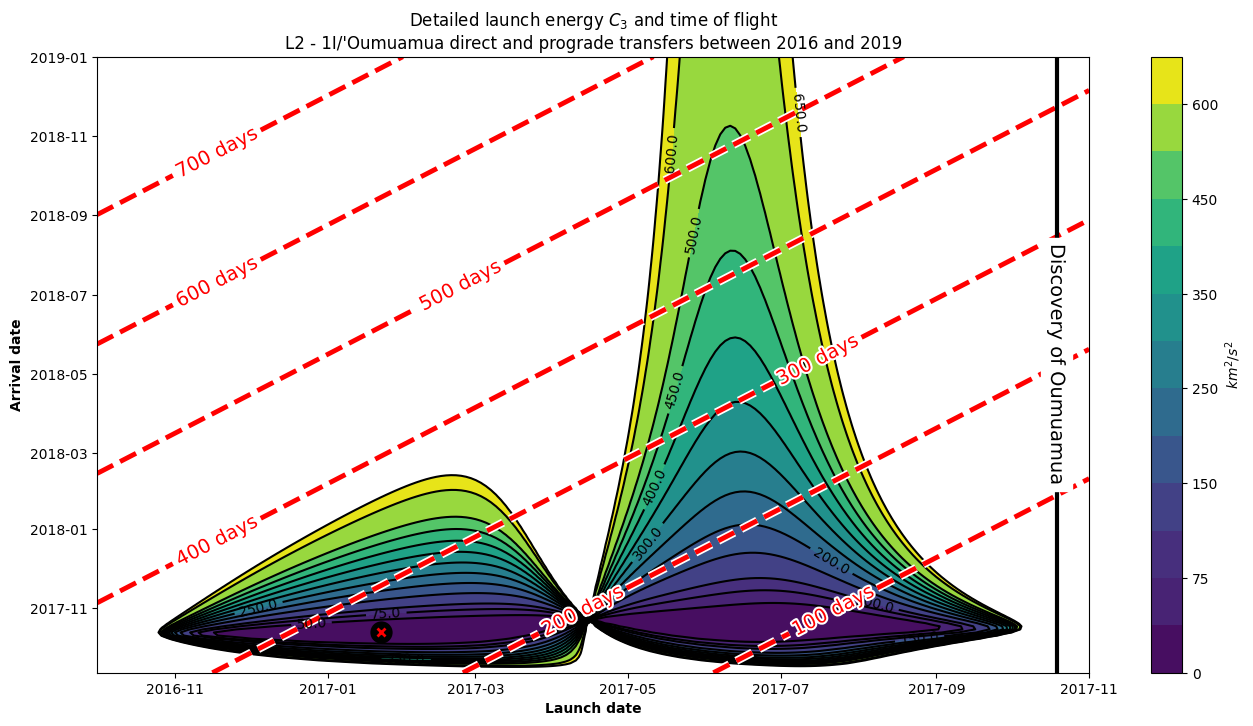
\includegraphics[width=\textwidth]{fig/static/oumuamua/l2-direct-detailed-porkchop-tof.png}
    \caption{Direct transfer from L2}
    \label{fig:oumuamua-l2-transfer}
\end{figure}

\end{frame}
%---------------------------------------------------------

%---------------------------------------------------------
\begin{frame}
\frametitle{1I/'Oumuamua: summary of results}

\begin{table}[H]
  \centering
  \begin{tabular}{|c|c|c|}
    \hline
    $\Delta v$ launch Earth [km/s] & $\Delta v$ launch L2 [km/s] & Reduction [\%] \\
    \hline
    13.85                          & 3.80                        & 72.56          \\
    \hline
  \end{tabular}
  \caption{Launch energy comparison}
  \label{tab:oumuamua-summary-results-v-launch}
\end{table}

\begin{table}[H]
  \centering
  \begin{tabular}{|c|c|c|}
    \hline
    $\Delta V$ arrival Earth [km/s] & $\Delta V$ arrival L2 [km/s] & Reduction [\%] \\
    \hline
    62.33                           & 61.46                        & 1.40           \\
    \hline
  \end{tabular}
  \caption{Arrival velocity comparison}
  \label{tab:oumuamua-summary-results-arrival-v}
\end{table}

\begin{table}[H]
  \centering
  \begin{tabular}{|c|c|c|}
    \hline
    $C_3$ launch Earth [km$^2$/s$^2$] & $C_3$ launch L2 [km$^2$/s$^2$] & Reduction [\%] \\
    \hline
    192.00                            & 14.41                          & 92.51          \\
    \hline
  \end{tabular}
  \caption{Characteristic energy comparison}
  \label{tab:oumuamua-summary-results-c3-launch}
\end{table}

\end{frame}
%---------------------------------------------------------

%---------------------------------------------------------
\begin{frame}
\frametitle{2I/Borisov: direct prograde transfer from Earth}

\begin{figure}[h]
    \centering
    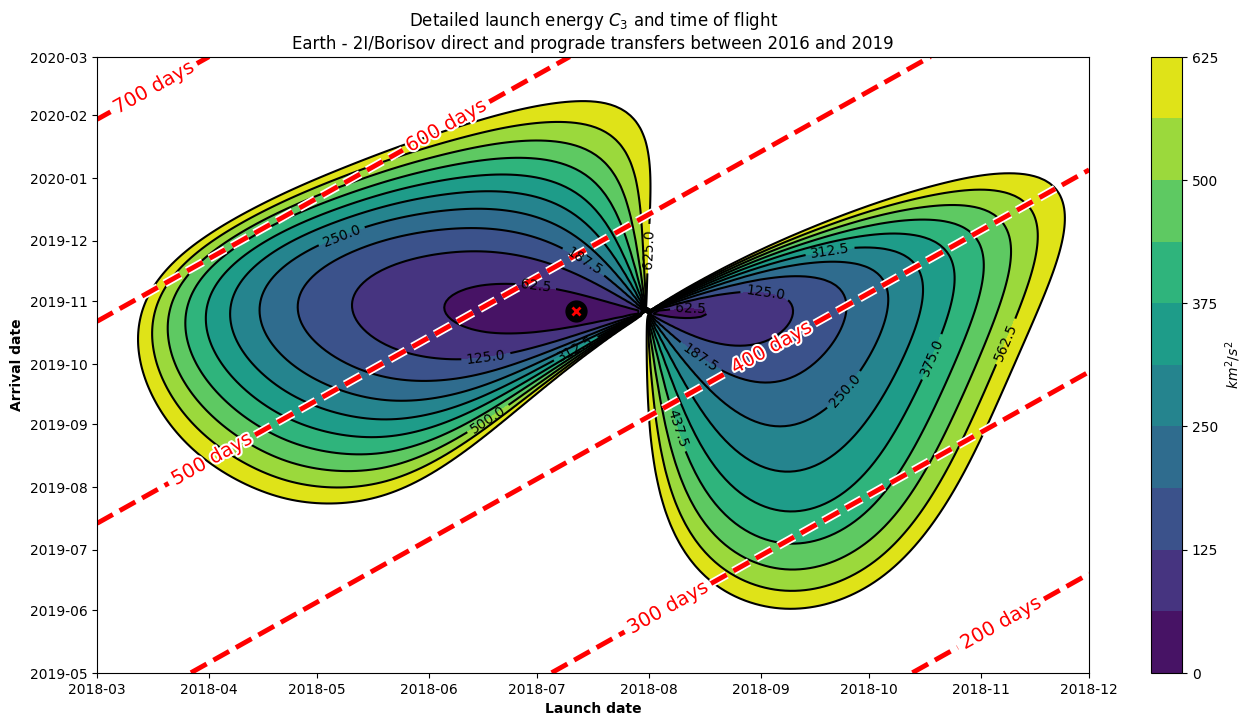
\includegraphics[width=\textwidth]{fig/static/borisov/direct-detailed-porkchop-tof.png}
    \caption{Direct transfer from Earth}
    \label{fig:borisov-earth-transfer}
\end{figure}

\end{frame}
%---------------------------------------------------------

%---------------------------------------------------------
\begin{frame}
\frametitle{2I/Borisov: direct prograde transfer from L2}

\begin{figure}[h]
    \centering
    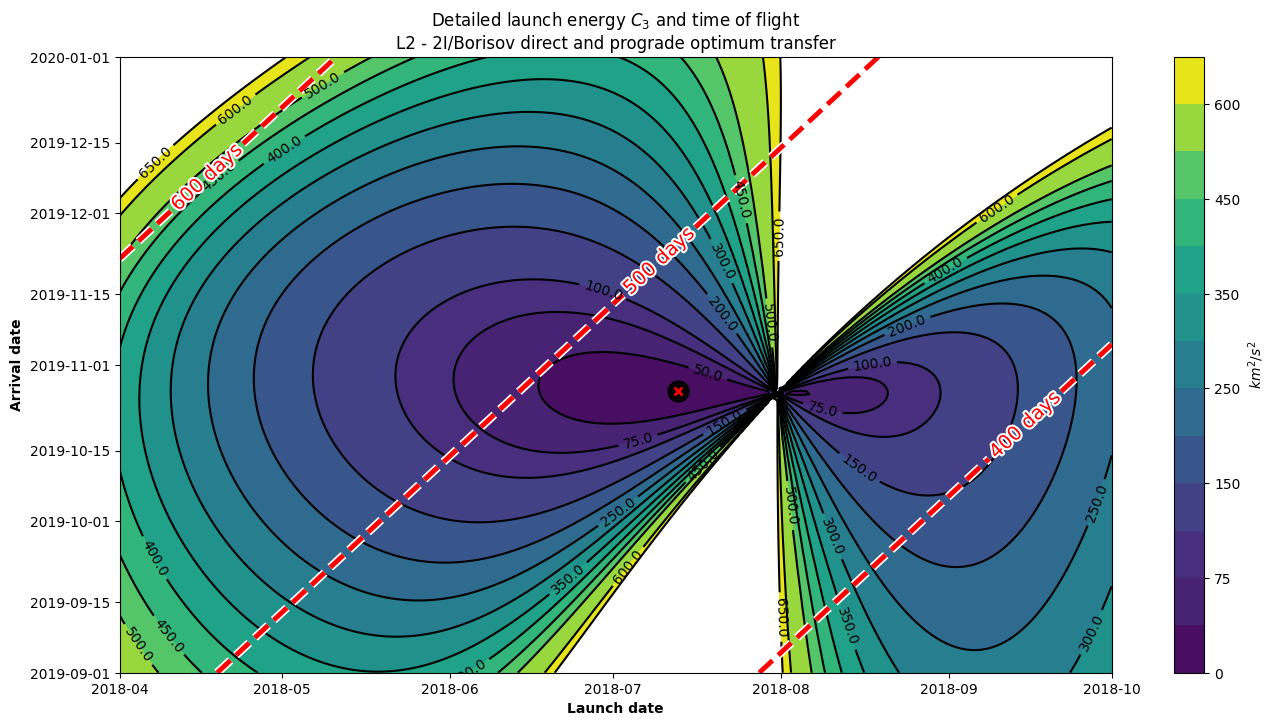
\includegraphics[width=\textwidth]{fig/static/borisov/l2-direct-detailed-porkchop-tof.png}
    \caption{Direct transfer from Earth}
    \label{fig:borisov-l2-transfer}
\end{figure}

\end{frame}
%---------------------------------------------------------

%---------------------------------------------------------
\begin{frame}
\frametitle{2I/Borisov: summary of results}

\begin{table}[H]
  \centering
  \begin{tabular}{|c|c|c|}
    \hline
    $\Delta v$ launch Earth [km/s] & $\Delta v$ launch L2 [km/s] & Reduction [\%] \\
    \hline
    16.90                          & 5.85                        & 65.38          \\
    \hline
  \end{tabular}
  \caption{Launch energy comparison}
  \label{tab:borisov-summary-results-v-launch}
\end{table}

\begin{table}[H]
  \centering
  \begin{tabular}{|c|c|c|}
    \hline
    $\Delta V$ arrival Earth [km/s] & $\Delta V$ arrival L2 [km/s] & Reduction [\%] \\
    \hline
    33.00                           & 33.02                        & -0.06          \\
    \hline
  \end{tabular}
  \caption{Arrival velocity comparison}
  \label{tab:borisov-summary-results-arrival-v}
\end{table}

\begin{table}[H]
  \centering
  \begin{tabular}{|c|c|c|}
    \hline
    $C_3$ launch Earth [km$^2$/s$^2$] & $C_3$ launch L2 [km$^2$/s$^2$] & Reduction [\%] \\
    \hline
    286.00                            & 34.30                          & 88.08          \\
    \hline
  \end{tabular}
  \caption{Characteristic energy comparison}
  \label{tab:borisov-summary-results-c3-launch}
\end{table}

\end{frame}
%---------------------------------------------------------

%---------------------------------------------------------
\begin{frame}
\frametitle{Conclusions}

\begin{block}{L2 as the optimal launching point}
Launching an intercepting spacecraft from L2 is more fuel efficient. These
results agree with the ones presented by the Comet Interceptor mission.
\end{block}

\pause

\vspace{0.5cm}
\begin{block}{A direct transfer is possible}
Existing propulsive technologies allow for a direct transfer from Earth to an
ISO with similar characteristics to 1I/'Oumuamua and 2I/Borisov.
\end{block}

\pause

\vspace{0.5cm}
\begin{block}{Need of increased vigilance in the search for ISOs}
Both optimum transfer dates take place prior the discovery of 1I/'Oumuamua and
2I/Borisov. Surveillance of the sky is crucial to detect future ISOs.
\end{block}

\end{frame}
%---------------------------------------------------------

%---------------------------------------------------------
\begin{frame}
\frametitle{Future work}

\begin{exampleblock}{Generating a synthetic population of ISOs}
Synthetic orbits of ISOs can be generated by using Monte-Carlo simulations.
This could allow to predict future ISO encounters.
\end{exampleblock}

\pause
\vspace{0.5cm}
\begin{exampleblock}{Drafting optimum transfers}
Optimum transfers can be solved for previous synthetic data. Solutions would be
used by future missions parked at L2.
\end{exampleblock}

\pause
\vspace{0.5cm}
\begin{exampleblock}{Trajectory optimization}
A combination of multiple gravity assists and deep space maneuvers may allow for
a more efficient transfer to an ISO, depending on the scenario.
\end{exampleblock}

\end{frame}
%---------------------------------------------------------

%---------------------------------------------------------
\begin{frame}
\frametitle{References}

\begin{alertblock}{Official repository}
\vspace{0.2cm}
This work is hosted in \textbf{\href{https://github.com/jorgepiloto/tfm}{https://github.com/jorgepiloto/tfm}}
\vspace{0.2cm}
\end{alertblock}

\end{frame}
%---------------------------------------------------------

%---------------------------------------------------------
\begin{frame}
\frametitle{Additional materials: 1I/'Oumuamua shape}

\begin{figure}[h]
    \centering
    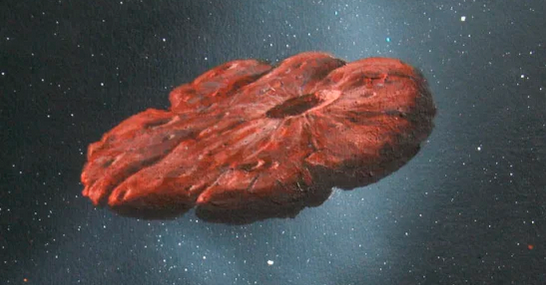
\includegraphics[width=\textwidth]{fig/static/oumuamua-shape.png}
        \caption{1I/'Oumuamua shape\\\tiny{Illustration by William Hartmann/Michael Belton/AP}}
    \label{fig:oumuamua-shape}
\end{figure}

\end{frame}
%---------------------------------------------------------

%---------------------------------------------------------
\begin{frame}
\frametitle{Additional materials: ISEE-3 mission}

\begin{figure}[h]
    \centering
    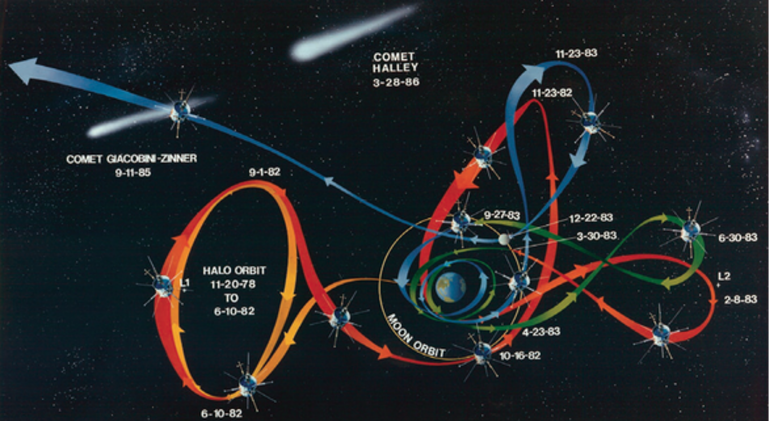
\includegraphics[width=\textwidth]{fig/static/isee-mission.png}
        \caption{ISEE-3 mission\\\tiny{Illustration by NASA}}
    \label{fig:isee-mission}
\end{figure}

\end{frame}
%---------------------------------------------------------

%---------------------------------------------------------
\begin{frame}
\frametitle{Additional materials: NEO surveyor}

\begin{figure}[h]
    \centering
    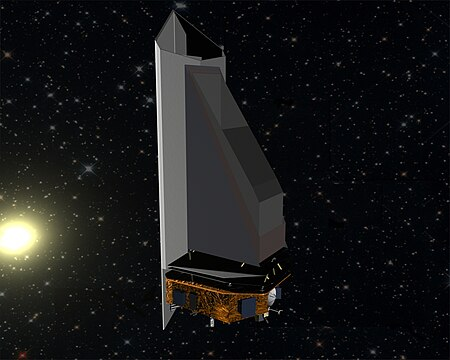
\includegraphics[width=0.65\textwidth]{fig/static/neo-surveyor.jpg}
        \caption{NEO surveyor\\\tiny{Illustration by NASA}}
    \label{fig:isee-mission}
\end{figure}

\end{frame}
%---------------------------------------------------------

%---------------------------------------------------------
\begin{frame}
\frametitle{Additional materials: Large Synoptic Survey Telescope}

\begin{figure}[h]
    \centering
    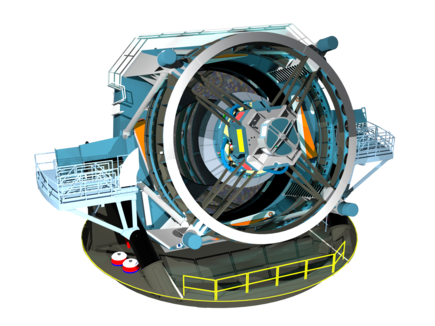
\includegraphics[width=0.75\textwidth]{fig/static/lsst.png}
        \caption{LSST\\\tiny{Illustration by LSST Project Office}}
    \label{fig:lsst}
\end{figure}

\end{frame}
%---------------------------------------------------------





\end{document}
